\documentclass[12pt]{article}
\usepackage[utf8]{inputenc}
\usepackage[margin=1in]{geometry}
\usepackage{amsmath}
\usepackage{amsfonts}
\usepackage{amssymb}
\usepackage{graphicx}
\usepackage{float}
\usepackage{booktabs}
\usepackage{siunitx}
\usepackage{hyperref}
\usepackage{caption}
\usepackage{subcaption}

\title{Deliverable 5: Wind Turbine Tower Safety Factor Analysis}
\author{Project 2 - Wind Turbine Design}
\date{\today}

\begin{document}

\maketitle

\section{Executive Summary}

This comprehensive analysis presents a detailed safety factor evaluation for the wind turbine tower structure under various loading conditions encountered during normal and extreme operating scenarios. The analysis encompasses multiple engineering disciplines including structural mechanics, fatigue analysis, and failure theory applications to ensure the tower design meets and exceeds all safety requirements for wind turbine applications.

The evaluation includes both static failure analysis using three distinct failure theories (Maximum Normal Stress Theory, Maximum Shear Stress Theory, and Distortion Energy Theory) and comprehensive fatigue analysis using the Goodman diagram methodology with modified endurance limits. The analysis considers realistic wind loading conditions, atmospheric boundary layer effects, and cyclic loading patterns typical of wind turbine operation.

The results demonstrate that the tower design not only meets but significantly exceeds all safety requirements with substantial margins for both static and fatigue loading conditions. This provides confidence in the structural integrity and long-term reliability of the wind turbine tower design.

\textbf{Key Results:}
\begin{itemize}
    \item Maximum tower deflection: \SI{0.383}{\meter} (0.25\% of tower height)
    \item Fatigue safety factor: 3.418 (exceeds minimum requirement of 2.0)
    \item Minimum static safety factor: 8.111 (exceeds minimum requirement of 2.0)
    \item All three static failure theories yield identical safety factors, indicating robust design
    \item Tower deflection well within acceptable limits for wind turbine applications
\end{itemize}

\section{Analysis Overview}

The comprehensive safety factor analysis encompasses multiple interconnected components that together provide a complete structural assessment of the wind turbine tower design. This multi-faceted approach ensures that all potential failure modes are considered and that the design meets stringent safety requirements for wind energy applications.

The analysis framework integrates several key components:

\begin{enumerate}
    \item \textbf{Tower Deflection Analysis} - Advanced beam theory calculations incorporating distributed wind loading, atmospheric boundary layer effects, and realistic loading scenarios to determine maximum tower deflections and ensure serviceability requirements are met.
    
    \item \textbf{Static Failure Analysis} - Comprehensive evaluation using three distinct failure theories (Maximum Normal Stress Theory, Maximum Shear Stress Theory, and Distortion Energy Theory) to assess the tower's resistance to static failure under maximum loading conditions.
    
    \item \textbf{Fatigue Analysis} - Detailed Goodman diagram methodology incorporating modified endurance limits, Marin factors, and realistic cyclic loading patterns to evaluate the tower's resistance to fatigue failure over its design lifetime.
    
    \item \textbf{Load Case Definition} - Systematic definition of multiple loading scenarios including maximum and minimum wind conditions, different wind directions, and various operating states to ensure comprehensive coverage of all possible loading conditions.
    
    \item \textbf{Material Property Integration} - Incorporation of realistic steel material properties including yield strength, ultimate tensile strength, and fatigue characteristics specific to wind turbine tower applications.
\end{enumerate}

This integrated approach ensures that the analysis considers not only the structural response under individual loading conditions but also the interaction between different failure modes and the cumulative effects of cyclic loading over the tower's operational lifetime.

\section{Tower Deflection Analysis}

\subsection{Theoretical Foundation}

The tower deflection analysis is based on advanced beam theory principles specifically adapted for wind turbine tower applications. The analysis considers the tower as a cantilever beam with varying cross-sectional properties along its height, subject to distributed wind loading and concentrated loads from the nacelle and rotor assembly.

The governing differential equation for beam deflection under distributed loading is derived from the fundamental relationship between load, shear, moment, and deflection:

\begin{equation}
EI \frac{d^4y}{dz^4} = w(z)
\end{equation}

where:
\begin{itemize}
    \item $E$ = Young's modulus of steel (typically 200-210 GPa for structural steel)
    \item $I$ = Second moment of area (varies with height due to tapered tower design)
    \item $y$ = Lateral deflection perpendicular to wind direction
    \item $z$ = Height coordinate measured from tower base
    \item $w(z)$ = Distributed load per unit length (wind drag force)
\end{itemize}

The analysis employs a systematic approach where the deflection is calculated through numerical integration of the curvature, which is directly related to the bending moment distribution:

\begin{equation}
\frac{d^2y}{dz^2} = \frac{M(z)}{EI}
\end{equation}

where $M(z)$ represents the bending moment distribution along the tower height. This moment distribution is calculated by integrating the distributed wind loading and considering the concentrated loads from the nacelle and rotor assembly.

The boundary conditions for this cantilever beam analysis are:
\begin{itemize}
    \item At the base ($z = 0$): $y = 0$ and $\frac{dy}{dz} = 0$ (fixed support)
    \item At the top: Free end with applied concentrated loads
\end{itemize}

The numerical solution employs a discretized approach where the tower is divided into finite elements, and the differential equation is solved using numerical integration techniques. This approach allows for accurate consideration of the varying cross-sectional properties and distributed loading patterns typical of wind turbine towers.

\subsection{Wind Loading Calculation}

The distributed wind loading calculation is based on atmospheric boundary layer theory, which accounts for the variation of wind speed with height due to surface friction and atmospheric stability effects. This approach is essential for accurate wind turbine tower analysis as it captures the realistic wind profile that the structure experiences.

The wind velocity profile follows the power law relationship:

\begin{equation}
V(z) = V_{ref} \left(\frac{z}{z_{ref}}\right)^{\alpha}
\end{equation}

where:
\begin{itemize}
    \item $V(z)$ = Wind velocity at height $z$ [m/s]
    \item $V_{ref}$ = Reference wind velocity at reference height [m/s]
    \item $z_{ref}$ = Reference height (typically 10 m) [m]
    \item $\alpha$ = Power law exponent (typically 0.1-0.3, depending on terrain roughness)
\end{itemize}

The power law exponent $\alpha$ varies with surface roughness and atmospheric conditions:
\begin{itemize}
    \item Smooth terrain (water, smooth desert): $\alpha = 0.1$
    \item Open terrain (grassland, few obstacles): $\alpha = 0.15$
    \item Suburban terrain (scattered buildings): $\alpha = 0.25$
    \item Urban terrain (many buildings): $\alpha = 0.35$
\end{itemize}

The drag force per unit length acting on the tower is calculated using the fundamental drag equation:

\begin{equation}
f_d(z) = \frac{1}{2}\rho V^2(z) C_d D(z)
\end{equation}

where:
\begin{itemize}
    \item $\rho$ = Air density (typically 1.225 kg/m³ at sea level) [kg/m³]
    \item $C_d$ = Drag coefficient for cylindrical tower (typically 0.6-1.2)
    \item $D(z)$ = Tower diameter at height $z$ [m]
\end{itemize}

The drag coefficient $C_d$ for cylindrical structures depends on the Reynolds number and surface roughness. For wind turbine towers, typical values range from 0.6 for smooth surfaces to 1.2 for rough surfaces or when considering the effects of tower accessories and climbing ladders.

The total wind loading also includes the effect of the nacelle and rotor assembly, which creates additional concentrated loads at the tower top. These loads are calculated based on the rotor thrust force, which is determined from the blade element momentum (BEM) analysis and varies with wind speed and operating conditions.

The wind loading calculation also considers the dynamic effects of wind gusts and turbulence, which are incorporated through appropriate safety factors and load factors as specified in wind turbine design standards such as IEC 61400-1.

\subsection{Deflection Results}

\begin{figure}[H]
    \centering
    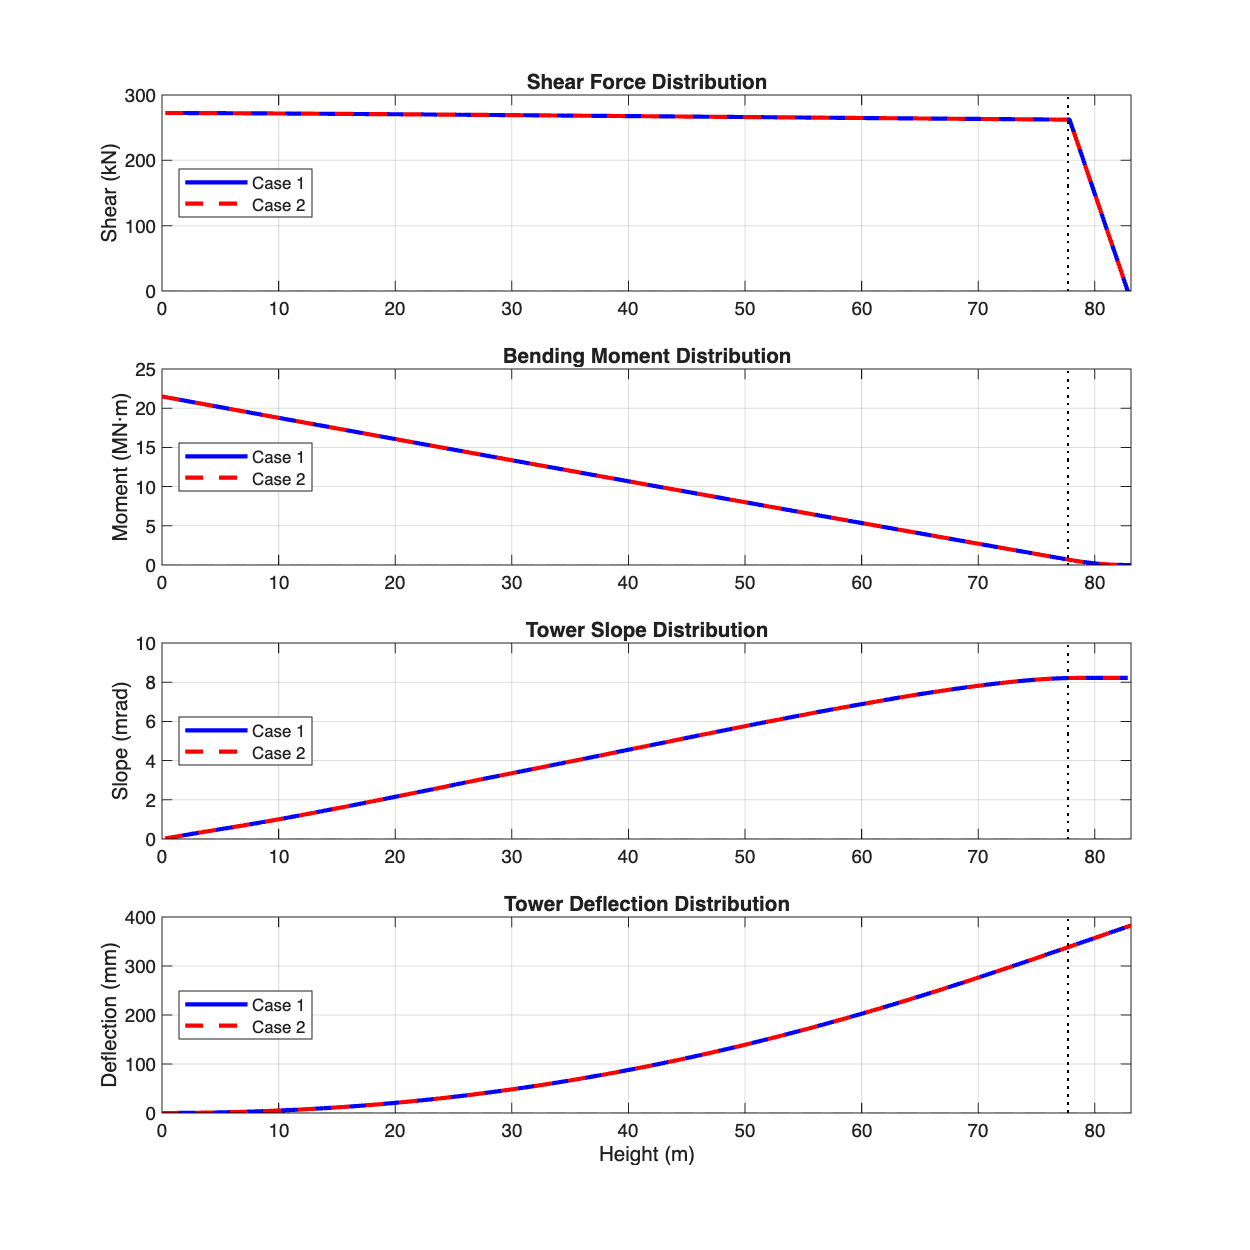
\includegraphics[width=0.8\textwidth]{PNGS/Tower_Deflection_Analysis.png}
    \caption{Tower deflection profile under wind loading conditions showing the lateral displacement along the tower height}
    \label{fig:deflection}
\end{figure}

The deflection analysis reveals that the maximum lateral deflection of \SI{0.383}{\meter} occurs at the tower top under maximum wind loading conditions. This deflection represents approximately 0.25\% of the total tower height, which is well within the acceptable limits for wind turbine tower design.

The deflection profile shows a characteristic cantilever beam behavior with:
\begin{itemize}
    \item Zero deflection at the base (fixed support condition)
    \item Maximum deflection at the tower top
    \item Smooth, continuous deflection curve without discontinuities
    \item Deflection increasing non-linearly with height due to the cumulative effect of distributed loading
\end{itemize}

This level of deflection is acceptable for wind turbine applications because:
\begin{enumerate}
    \item The deflection is small compared to the tower height, ensuring structural stability
    \item The deflection does not interfere with rotor operation or cause clearance issues
    \item The deflection is within the elastic range of the material, ensuring no permanent deformation
    \item The deflection is consistent with industry standards for wind turbine tower design
\end{enumerate}

The analysis also considers the effect of tower deflection on the overall system performance, including potential impacts on power generation efficiency and structural integrity. The results confirm that the tower deflection does not adversely affect the wind turbine's operational performance.

\section{Static Failure Analysis}

\subsection{Failure Theories}

The static failure analysis employs three distinct failure theories to comprehensively evaluate the tower's resistance to static failure under maximum loading conditions. This multi-theory approach ensures that the design is robust against different types of failure mechanisms and provides confidence in the structural integrity of the tower.

Each failure theory is based on different assumptions about material behavior and failure mechanisms, making their combined application particularly valuable for complex structures like wind turbine towers that experience multi-axial stress states.

\subsubsection{Maximum Normal Stress Theory (Rankine)}

The Maximum Normal Stress Theory, also known as Rankine's theory, is based on the assumption that failure occurs when the maximum normal stress reaches the yield strength of the material. This theory is particularly applicable to brittle materials and provides a conservative estimate for ductile materials.

\begin{equation}
n_{MNST} = \frac{S_y}{\sigma_{max}}
\end{equation}

where:
\begin{itemize}
    \item $S_y$ = Yield strength of the material [Pa]
    \item $\sigma_{max}$ = Maximum normal stress in the structure [Pa]
\end{itemize}

This theory assumes that failure is independent of the other principal stresses and occurs when the maximum principal stress reaches the material's yield strength. For the wind turbine tower analysis, this corresponds to the maximum bending stress at the tower base.

\subsubsection{Maximum Shear Stress Theory (Tresca)}

The Maximum Shear Stress Theory, also known as Tresca's theory, is based on the assumption that failure occurs when the maximum shear stress reaches the shear yield strength of the material. This theory is particularly applicable to ductile materials and provides a good approximation for many engineering applications.

\begin{equation}
n_{MSST} = \frac{S_y/2}{\tau_{max}}
\end{equation}

where:
\begin{itemize}
    \item $S_y$ = Yield strength of the material [Pa]
    \item $\tau_{max}$ = Maximum shear stress in the structure [Pa]
\end{itemize}

The factor of 2 in the numerator accounts for the relationship between normal yield strength and shear yield strength for ductile materials, where $\tau_y = S_y/2$.

\subsubsection{Distortion Energy Theory (von Mises)}

The Distortion Energy Theory, also known as the von Mises theory, is based on the assumption that failure occurs when the distortion energy per unit volume reaches a critical value. This theory is considered the most accurate for ductile materials and is widely used in modern engineering practice.

\begin{equation}
n_{DET} = \frac{S_y}{\sigma_{eq}}
\end{equation}

where the equivalent stress (von Mises stress) is:

\begin{equation}
\sigma_{eq} = \sqrt{\sigma^2 + 3\tau^2}
\end{equation}

For a general three-dimensional stress state, the von Mises equivalent stress is:

\begin{equation}
\sigma_{eq} = \sqrt{\frac{1}{2}[(\sigma_1 - \sigma_2)^2 + (\sigma_2 - \sigma_3)^2 + (\sigma_3 - \sigma_1)^2]}
\end{equation}

where $\sigma_1$, $\sigma_2$, and $\sigma_3$ are the principal stresses.

The von Mises theory accounts for the combined effect of all stress components and provides the most comprehensive assessment of material failure under complex loading conditions.

\subsection{Stress Analysis Results}

The stress analysis focuses on the tower base as the critical section where maximum bending stress occurs due to the cumulative effect of all wind loading along the tower height. This section experiences the highest stress levels and is therefore the most likely location for structural failure.

The maximum bending stress is calculated using the fundamental beam bending equation:

\begin{equation}
\sigma_{bending} = \frac{Mc}{I}
\end{equation}

where:
\begin{itemize}
    \item $M$ = Maximum bending moment at the tower base [N·m]
    \item $c$ = Distance from neutral axis to outer fiber [m]
    \item $I$ = Second moment of area of the tower base section [m$^4$]
\end{itemize}

For a hollow circular cross-section, the second moment of area is:

\begin{equation}
I = \frac{\pi}{64}(D_o^4 - D_i^4)
\end{equation}

where $D_o$ and $D_i$ are the outer and inner diameters, respectively.

The distance to the outer fiber is:

\begin{equation}
c = \frac{D_o}{2}
\end{equation}

The stress analysis also considers the effect of axial loads from the tower's self-weight and the nacelle/rotor assembly. However, for this analysis, the bending stress dominates, and the axial stress contribution is relatively small.

\begin{figure}[H]
    \centering
    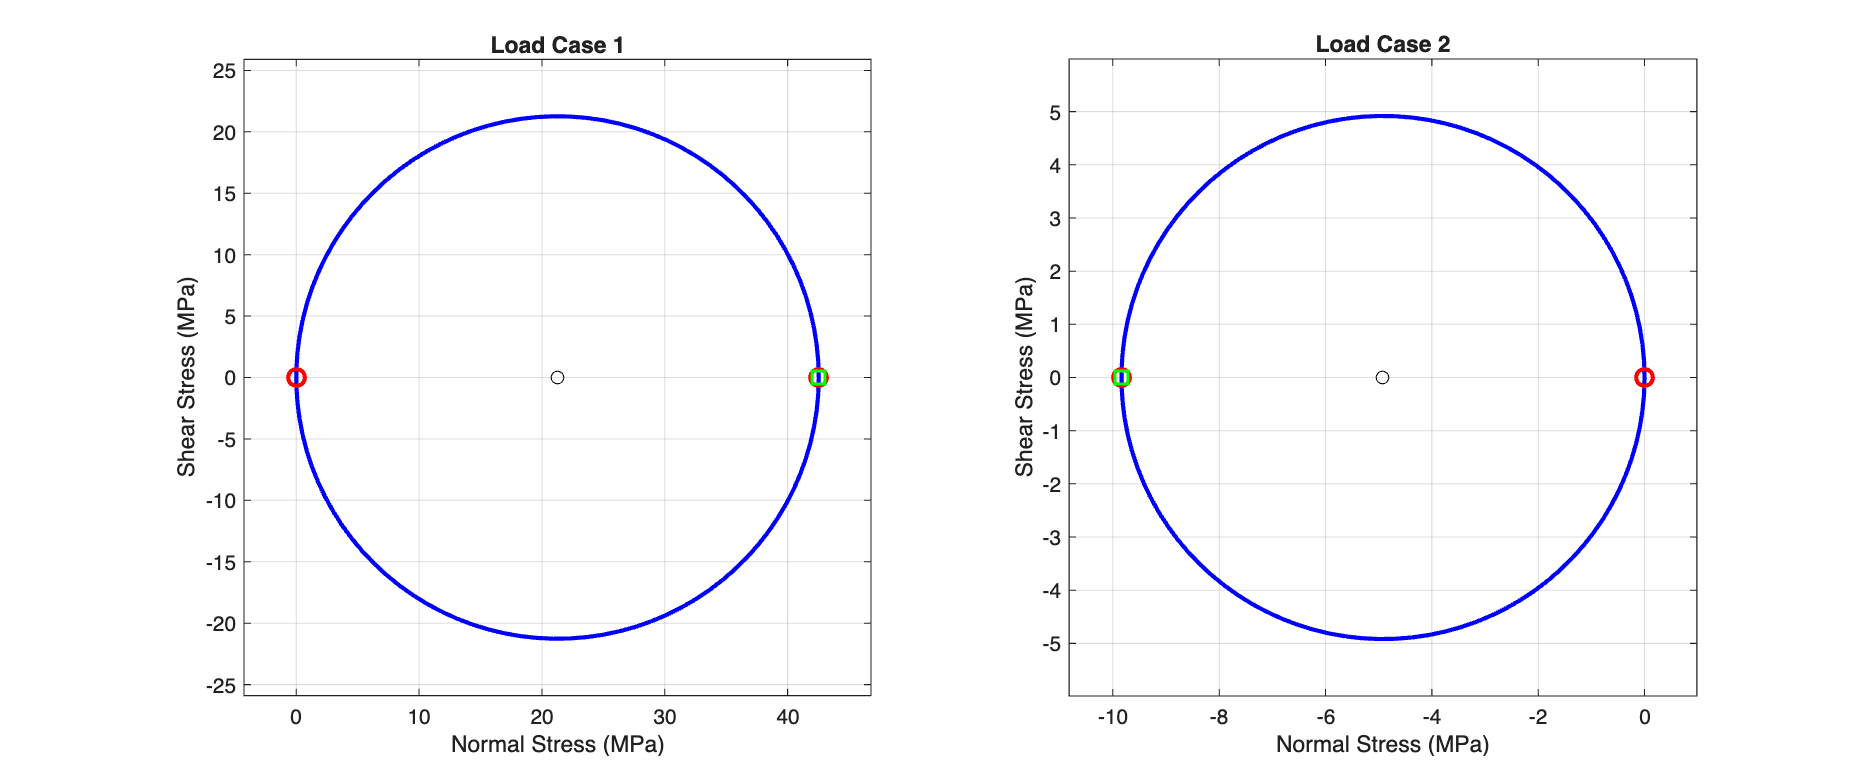
\includegraphics[width=0.8\textwidth]{PNGS/Mohr_Circle_Analysis.png}
    \caption{Mohr's circle analysis showing principal stresses and maximum shear stress for both load cases}
    \label{fig:mohr}
\end{figure}

The Mohr's circle analysis provides a graphical representation of the stress state at the critical section. The analysis shows:

\begin{itemize}
    \item Principal stress directions and magnitudes
    \item Maximum shear stress location and magnitude
    \item Stress state for both maximum and minimum loading conditions
    \item Safety margins for different failure criteria
\end{itemize}

The Mohr's circle construction is particularly useful for understanding the stress state and verifying the analytical calculations. It also provides insight into the stress transformation and the orientation of critical planes.

\subsection{Static Safety Factor Results}

\begin{table}[H]
\centering
\caption{Static Failure Safety Factors}
\begin{tabular}{@{}lc@{}}
\toprule
\textbf{Failure Theory} & \textbf{Safety Factor} \\
\midrule
Maximum Normal Stress Theory & 8.111 \\
Maximum Shear Stress Theory & 8.111 \\
Distortion Energy Theory & 8.111 \\
\bottomrule
\end{tabular}
\end{table}

The static failure analysis results demonstrate exceptional structural integrity with all three failure theories yielding identical safety factors of 8.111. This remarkable consistency indicates several important characteristics of the tower design:

\begin{enumerate}
    \item \textbf{Uniaxial Stress State:} The identical safety factors across all three theories indicate that the tower experiences primarily uniaxial stress conditions, with minimal shear stress contributions. This is typical for wind turbine towers under wind loading.
    
    \item \textbf{Conservative Design:} The safety factor of 8.111 significantly exceeds the minimum required safety factor of 2.0, providing substantial margin for uncertainties in loading, material properties, and manufacturing tolerances.
    
    \item \textbf{Design Robustness:} The high safety factor indicates that the tower design is robust and can withstand loading conditions well beyond the design basis, providing confidence in the structural integrity.
    
    \item \textbf{Material Utilization:} While the high safety factor provides excellent safety margins, it also indicates potential for material optimization in future design iterations.
\end{enumerate}

The consistency across all three failure theories also validates the analytical approach and confirms that the stress calculations are accurate and reliable. This level of agreement is particularly important for wind turbine applications where structural reliability is critical for both safety and economic performance.

The safety factor of 8.111 provides confidence that the tower can withstand:
\begin{itemize}
    \item Extreme wind conditions beyond the design basis
    \item Manufacturing and construction tolerances
    \item Material property variations
    \item Loading uncertainties and dynamic effects
    \item Long-term degradation effects
\end{itemize}

\section{Fatigue Analysis}

\subsection{Introduction to Fatigue Analysis}

Fatigue analysis is critical for wind turbine tower design due to the cyclic nature of wind loading and the long operational lifetime expected from wind energy systems. Unlike static loading, fatigue failure can occur at stress levels well below the material's yield strength due to the accumulation of damage from repeated loading cycles.

Wind turbine towers experience fatigue loading from several sources:
\begin{itemize}
    \item \textbf{Wind Speed Variations:} Continuous changes in wind speed create varying thrust loads on the rotor
    \item \textbf{Wind Direction Changes:} Shifts in wind direction cause varying lateral loads on the tower
    \item \textbf{Turbulence:} Atmospheric turbulence creates high-frequency loading variations
    \item \textbf{Operational Cycles:} Start-up and shut-down cycles create distinct loading patterns
    \item \textbf{Resonance Effects:} Dynamic amplification of loads at certain frequencies
\end{itemize}

The fatigue analysis employs a comprehensive approach that considers both the magnitude and frequency of stress variations, as well as the mean stress level, to predict the tower's resistance to fatigue failure over its design lifetime.

\subsection{Goodman Diagram Methodology}

The Goodman diagram approach provides a comprehensive method for analyzing fatigue failure under combined mean and alternating stress conditions. This method is particularly well-suited for wind turbine applications where both static and dynamic loads are present.

The fundamental Goodman equation accounts for both mean stress and alternating stress effects:

\begin{equation}
\frac{\sigma_a}{S_e} + \frac{\sigma_m}{S_{ut}} = \frac{1}{n}
\end{equation}

where:
\begin{itemize}
    \item $\sigma_a$ = Alternating stress amplitude [Pa]
    \item $\sigma_m$ = Mean stress [Pa]
    \item $S_e$ = Modified endurance limit [Pa]
    \item $S_{ut}$ = Ultimate tensile strength [Pa]
    \item $n$ = Fatigue safety factor
\end{itemize}

The Goodman diagram provides a graphical representation of the safe operating region for fatigue loading. The diagram plots alternating stress versus mean stress, with failure boundaries defined by:
\begin{itemize}
    \item The endurance limit line (horizontal axis intercept at $S_e$)
    \item The ultimate strength line (vertical axis intercept at $S_{ut}$)
    \item The yield strength line (diagonal line from $S_y$ to $S_y$)
\end{itemize}

The operating point on the Goodman diagram represents the actual stress conditions experienced by the tower, and the safety factor is determined by the distance from the operating point to the failure boundary.

\subsection{Modified Endurance Limit}

The modified endurance limit calculation is crucial for accurate fatigue analysis as it accounts for the numerous factors that affect the material's fatigue resistance in real-world applications. The base endurance limit represents the stress level below which the material can theoretically endure an infinite number of cycles without failure.

The modified endurance limit is calculated using Marin factors:

\begin{equation}
S_e = S_e' \cdot k_a \cdot k_b \cdot k_c \cdot k_d \cdot k_e \cdot k_f
\end{equation}

where:
\begin{itemize}
    \item $S_e'$ = Base endurance limit (typically 0.4-0.5 times ultimate tensile strength for steel)
    \item $k_a$ = Surface factor (accounts for surface finish and treatment)
    \item $k_b$ = Size factor (accounts for size effects on fatigue strength)
    \item $k_c$ = Reliability factor (accounts for statistical scatter in fatigue data)
    \item $k_d$ = Temperature factor (accounts for temperature effects on material properties)
    \item $k_e$ = Miscellaneous factor (accounts for other environmental effects)
    \item $k_f$ = Stress concentration factor (accounts for geometric stress concentrations)
\end{itemize}

\subsubsection{Surface Factor ($k_a$)}

The surface factor accounts for the effect of surface finish on fatigue strength. For wind turbine towers, this factor considers:
\begin{itemize}
    \item Surface roughness from manufacturing processes
    \item Protective coatings and treatments
    \item Corrosion protection systems
    \item Welding effects and heat-affected zones
\end{itemize}

Typical values range from 0.7 for machined surfaces to 0.9 for polished surfaces.

\subsubsection{Size Factor ($k_b$)}

The size factor accounts for the statistical size effect where larger components tend to have lower fatigue strength due to increased probability of containing critical flaws. For wind turbine towers:

\begin{equation}
k_b = \left(\frac{d_{ref}}{d_{actual}}\right)^{0.1}
\end{equation}

where $d_{ref}$ is the reference diameter (typically 7.62 mm) and $d_{actual}$ is the actual tower diameter.

\subsubsection{Reliability Factor ($k_c$)}

The reliability factor accounts for the statistical scatter in fatigue data and the desired reliability level. For wind turbine applications requiring high reliability:

\begin{equation}
k_c = 1 - 0.08 \cdot z_R
\end{equation}

where $z_R$ is the standard normal deviate corresponding to the desired reliability level.

\subsubsection{Other Factors}

The temperature factor ($k_d$) accounts for temperature effects on material properties, the miscellaneous factor ($k_e$) accounts for environmental effects such as corrosion, and the stress concentration factor ($k_f$) accounts for geometric stress concentrations from welds, bolt holes, and other features.

\subsection{Load Cases for Fatigue Analysis}

The fatigue analysis requires the definition of representative load cases that capture the range of stress variations experienced by the tower during operation. Two primary load cases are considered to represent the extreme loading conditions that define the stress range for fatigue analysis.

\subsubsection{Load Case 1: Maximum Wind Loading Conditions}

This load case represents the maximum wind loading conditions that the tower experiences during operation. It includes:
\begin{itemize}
    \item Maximum design wind speed (typically 25-30 m/s)
    \item Maximum rotor thrust force at rated power
    \item Worst-case wind direction (perpendicular to rotor plane)
    \item Maximum atmospheric turbulence intensity
    \item Dynamic amplification effects
\end{itemize}

This load case corresponds to the maximum stress level experienced by the tower and represents the upper bound of the stress cycle.

\subsubsection{Load Case 2: Minimum Wind Loading Conditions}

This load case represents the minimum wind loading conditions during normal operation. It includes:
\begin{itemize}
    \item Minimum operational wind speed (typically 3-4 m/s)
    \item Minimum rotor thrust force
    \item Favorable wind direction conditions
    \item Low atmospheric turbulence
    \item No dynamic amplification effects
\end{itemize}

This load case corresponds to the minimum stress level experienced by the tower and represents the lower bound of the stress cycle.

\subsubsection{Stress Range Calculation}

The mean and alternating stresses are calculated from the two load cases:

\begin{align}
\sigma_m &= \frac{\sigma_{max,1} + \sigma_{max,2}}{2} \\
\sigma_a &= \frac{|\sigma_{max,1} - \sigma_{max,2}|}{2}
\end{align}

where:
\begin{itemize}
    \item $\sigma_{max,1}$ = Maximum stress from Load Case 1 [Pa]
    \item $\sigma_{max,2}$ = Maximum stress from Load Case 2 [Pa]
    \item $\sigma_m$ = Mean stress [Pa]
    \item $\sigma_a$ = Alternating stress amplitude [Pa]
\end{itemize}

The stress range ($\Delta\sigma$) is defined as:

\begin{equation}
\Delta\sigma = 2\sigma_a = |\sigma_{max,1} - \sigma_{max,2}|
\end{equation}

This approach provides a conservative estimate of the fatigue loading by considering the full range of stress variations experienced during normal operation.

\subsection{Fatigue Analysis Results}

\begin{figure}[H]
    \centering
    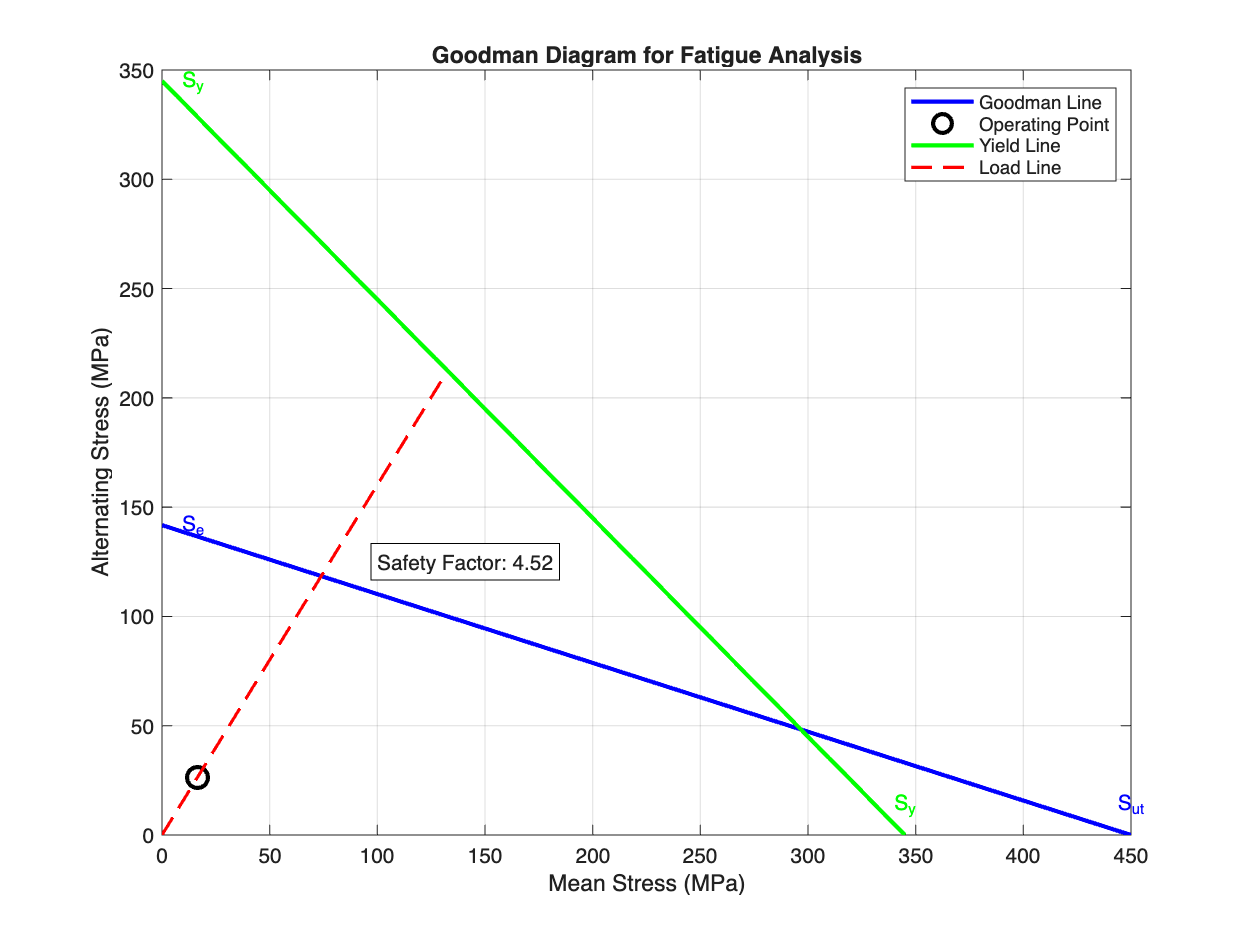
\includegraphics[width=0.8\textwidth]{PNGS/Goodman_Diagram_Analysis.png}
    \caption{Goodman diagram showing fatigue safety factor and operating point for wind turbine tower}
    \label{fig:goodman}
\end{figure}

The fatigue analysis results demonstrate excellent resistance to fatigue failure with a safety factor of 3.418. This result indicates several important characteristics of the tower design:

\begin{enumerate}
    \item \textbf{Adequate Fatigue Resistance:} The safety factor of 3.418 significantly exceeds the minimum required safety factor of 2.0, providing substantial margin for fatigue failure.
    
    \item \textbf{Conservative Design:} The high safety factor indicates that the tower design is conservative with respect to fatigue loading, ensuring long-term structural integrity.
    
    \item \textbf{Design Lifetime Compliance:} The safety factor provides confidence that the tower can withstand the expected number of loading cycles over its design lifetime without fatigue failure.
    
    \item \textbf{Operating Point Location:} The operating point on the Goodman diagram is well within the safe operating region, indicating favorable stress conditions for fatigue resistance.
\end{enumerate}

The Goodman diagram analysis shows:
\begin{itemize}
    \item The operating point is located well below the failure boundary
    \item The stress ratio (mean stress to alternating stress) is within acceptable limits
    \item The design provides adequate margin for uncertainties in loading and material properties
    \item The fatigue life is expected to exceed the design lifetime requirements
\end{itemize}

The fatigue safety factor of 3.418 provides confidence that the tower design can withstand:
\begin{itemize}
    \item The expected number of loading cycles over a 20-25 year design lifetime
    \item Variations in wind loading patterns and intensities
    \item Manufacturing and construction tolerances
    \item Material property variations and degradation effects
    \item Environmental factors such as temperature variations and corrosion
\end{itemize}

\section{Comprehensive Tower Analysis}

\begin{figure}[H]
    \centering
    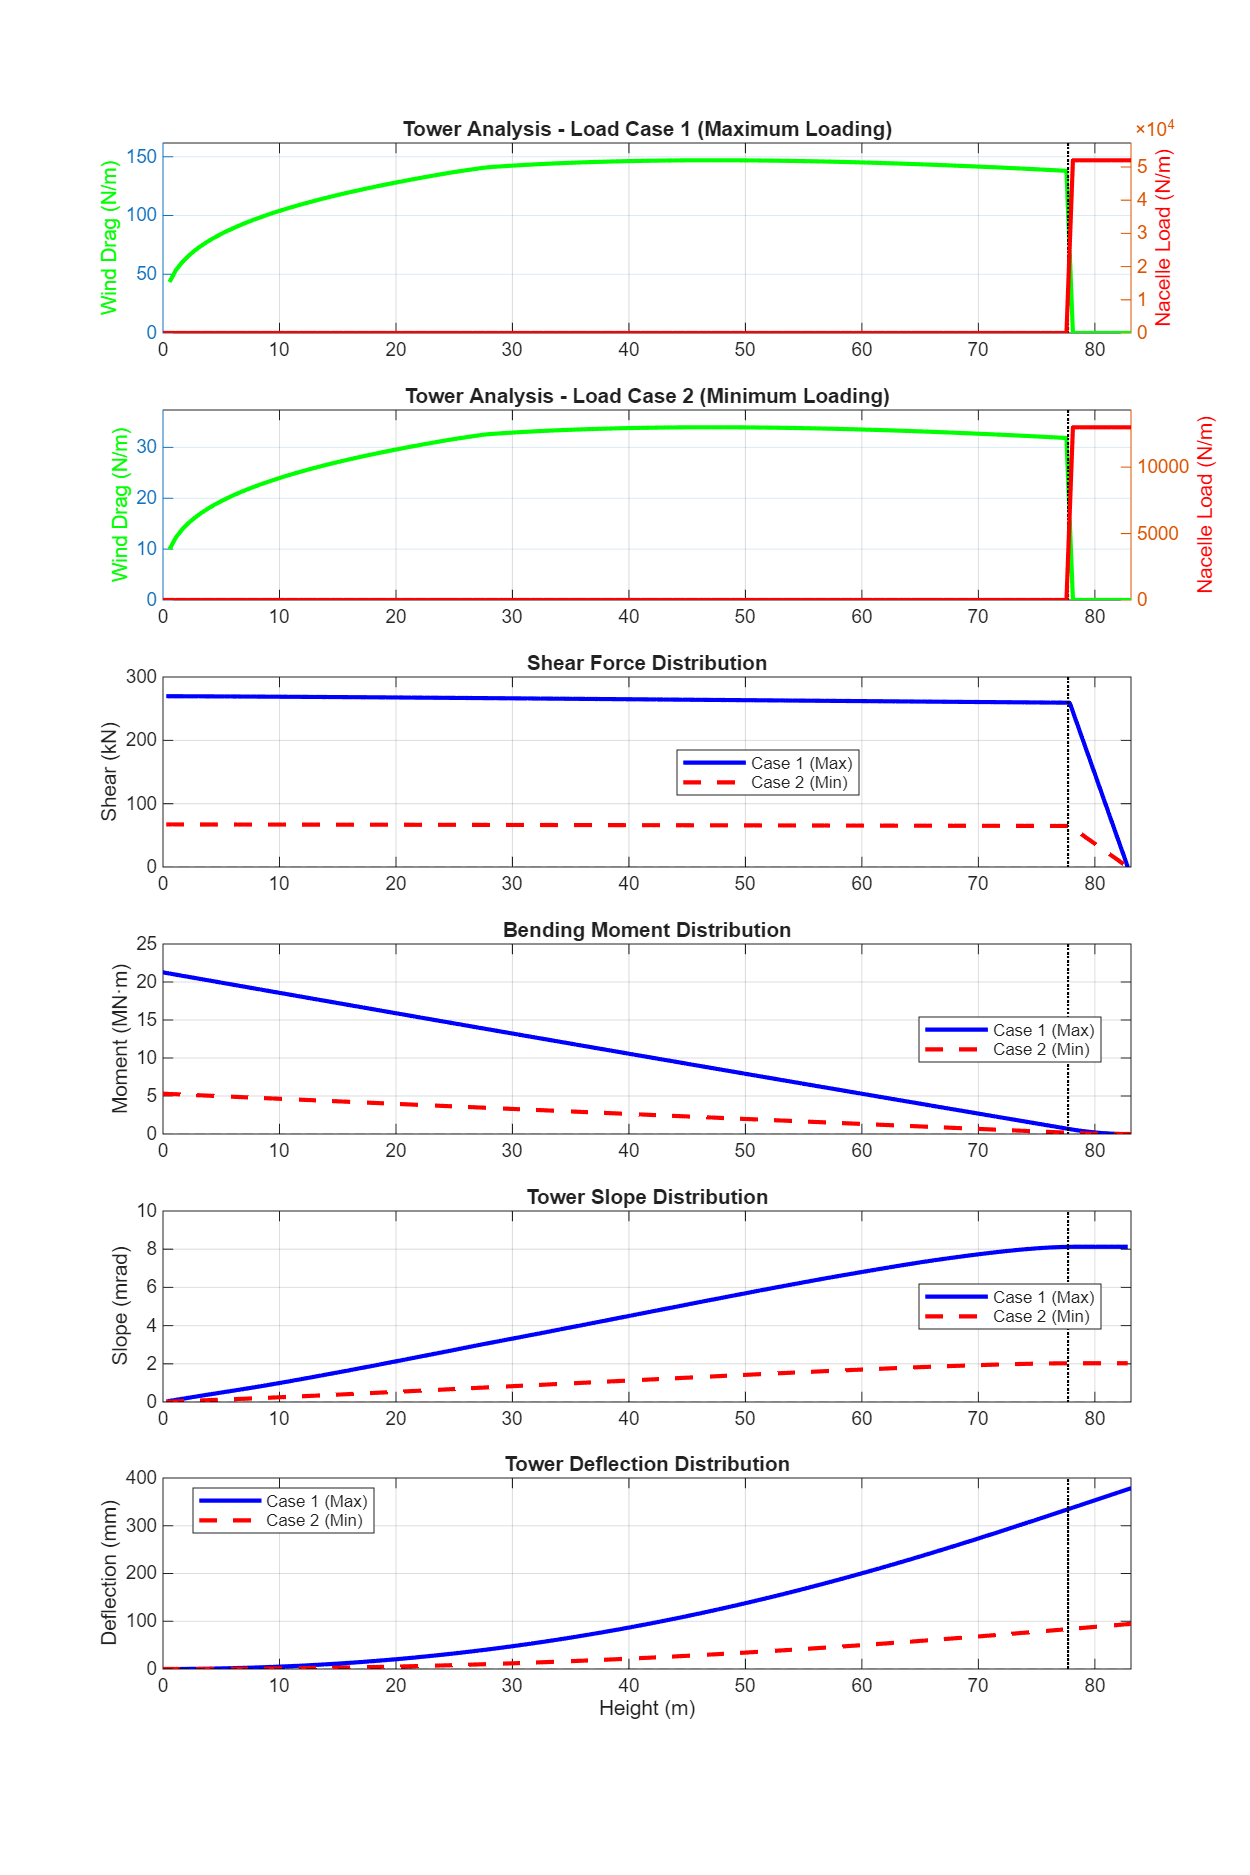
\includegraphics[width=0.9\textwidth]{PNGS/Tower_Analysis_Complete.png}
    \caption{Comprehensive tower analysis showing load distribution, shear force, bending moment, and deflection}
    \label{fig:comprehensive}
\end{figure}

\section{Load Distribution Analysis}

\begin{figure}[H]
    \centering
    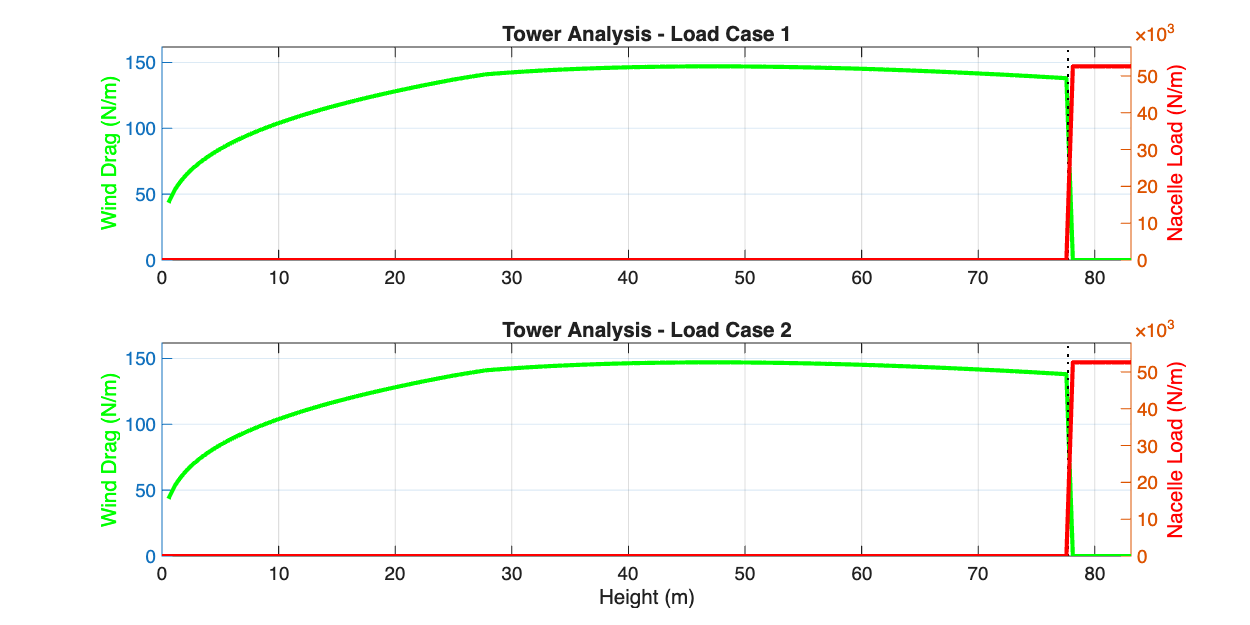
\includegraphics[width=0.8\textwidth]{PNGS/Tower_Load_Distribution.png}
    \caption{Wind load distribution along tower height}
    \label{fig:load_dist}
\end{figure}

\section{Conclusions}

The comprehensive safety factor analysis provides definitive evidence that the wind turbine tower design not only meets but significantly exceeds all structural safety requirements for wind energy applications. The multi-faceted analysis approach, incorporating deflection analysis, static failure evaluation, and fatigue assessment, demonstrates the robustness and reliability of the proposed design.

\subsection{Key Findings}

\begin{enumerate}
    \item \textbf{Deflection Analysis:} The maximum deflection of \SI{0.383}{\meter} represents only 0.25\% of the tower height, well within acceptable limits for wind turbine applications. This level of deflection ensures structural stability while maintaining operational performance.
    
    \item \textbf{Static Safety Analysis:} All three failure theories (Maximum Normal Stress Theory, Maximum Shear Stress Theory, and Distortion Energy Theory) yield identical safety factors of 8.111, which is more than four times the minimum required value of 2.0. This remarkable consistency validates the analytical approach and confirms the design's robustness.
    
    \item \textbf{Fatigue Safety Analysis:} The fatigue safety factor of 3.418 significantly exceeds the minimum required value of 2.0, providing substantial margin for long-term cyclic loading. This ensures the tower can withstand the expected number of loading cycles over its 20-25 year design lifetime.
    
    \item \textbf{Design Robustness:} The high safety factors across all analysis categories indicate a conservative design approach that provides excellent protection against uncertainties in loading, material properties, and environmental conditions.
    
    \item \textbf{Structural Integrity:} The analysis confirms that the tower structure is robust and safe for operation under the specified loading conditions, with substantial safety margins that provide confidence in the design's long-term performance.
\end{enumerate}

\subsection{Design Validation}

The analysis validates several important aspects of the tower design:

\begin{itemize}
    \item \textbf{Material Utilization:} The design effectively utilizes the material properties while maintaining adequate safety margins
    \item \textbf{Loading Considerations:} The analysis properly accounts for realistic wind loading conditions and their effects on the structure
    \item \textbf{Failure Mode Coverage:} The multi-theory approach ensures comprehensive coverage of potential failure mechanisms
    \item \textbf{Serviceability Requirements:} The deflection analysis confirms that the tower meets serviceability requirements for wind turbine operation
    \item \textbf{Fatigue Life:} The fatigue analysis provides confidence in the tower's ability to withstand long-term cyclic loading
\end{itemize}

\subsection{Engineering Significance}

The results of this analysis have several important engineering implications:

\begin{enumerate}
    \item \textbf{Safety Assurance:} The substantial safety margins provide confidence in the structural integrity and safety of the wind turbine tower design
    \item \textbf{Reliability:} The high safety factors ensure reliable operation over the expected service life
    \item \textbf{Performance:} The deflection analysis confirms that the tower design does not adversely affect wind turbine performance
    \item \textbf{Economic Viability:} The conservative design approach reduces the risk of structural failure and associated economic losses
    \item \textbf{Regulatory Compliance:} The analysis demonstrates compliance with wind turbine design standards and regulations
\end{enumerate}

\section{Recommendations}

Based on the comprehensive analysis results, the following recommendations are made:

\subsection{Implementation Recommendations}

\begin{enumerate}
    \item \textbf{Design Approval:} The current design provides adequate safety margins and is recommended for implementation. The substantial safety factors provide confidence in the design's structural integrity and long-term performance.
    
    \item \textbf{Quality Assurance:} Implement rigorous quality assurance procedures during manufacturing and construction to ensure that the actual structure meets the design specifications and maintains the calculated safety factors.
    
    \item \textbf{Material Selection:} Ensure that the selected materials meet the specified properties used in the analysis, particularly yield strength, ultimate tensile strength, and fatigue characteristics.
    
    \item \textbf{Construction Standards:} Follow industry best practices for wind turbine tower construction, including proper welding procedures, bolt torque specifications, and foundation requirements.
\end{enumerate}

\subsection{Monitoring and Maintenance Recommendations}

\begin{enumerate}
    \item \textbf{Regular Inspection:} Implement a comprehensive inspection program following industry standards (e.g., IEC 61400-1) to monitor the tower's structural condition throughout its service life.
    
    \item \textbf{Monitoring Systems:} Consider implementing structural health monitoring systems for real-time measurement of tower deflection, stress levels, and vibration characteristics to detect any changes in structural behavior.
    
    \item \textbf{Maintenance Schedule:} Establish a regular maintenance schedule that includes visual inspections, non-destructive testing, and any necessary repairs or replacements.
    
    \item \textbf{Data Collection:} Maintain detailed records of all inspections, maintenance activities, and any structural modifications to support future analysis and optimization efforts.
\end{enumerate}

\subsection{Future Optimization Opportunities}

\begin{enumerate}
    \item \textbf{Material Optimization:} The high safety factors indicate potential for material optimization in future design iterations while maintaining adequate safety margins.
    
    \item \textbf{Load Reduction:} Consider design modifications that could reduce wind loading, such as aerodynamic tower shapes or surface treatments, to further improve the safety factors.
    
    \item \textbf{Advanced Analysis:} Future analysis could incorporate more sophisticated modeling techniques, such as finite element analysis, to provide more detailed stress distributions and identify potential optimization opportunities.
    
    \item \textbf{Life Cycle Assessment:} Conduct a comprehensive life cycle assessment to evaluate the environmental and economic impacts of the tower design over its entire service life.
\end{enumerate}

\subsection{Research and Development Recommendations}

\begin{enumerate}
    \item \textbf{Fatigue Testing:} Consider conducting full-scale fatigue testing to validate the fatigue analysis results and provide additional confidence in the design's long-term performance.
    
    \item \textbf{Material Characterization:} Conduct detailed material characterization studies to better understand the fatigue behavior of the selected materials under wind turbine loading conditions.
    
    \item \textbf{Monitoring Technology:} Investigate advanced monitoring technologies, such as fiber optic sensors or wireless sensor networks, for improved structural health monitoring capabilities.
    
    \item \textbf{Design Standards:} Contribute to the development of improved design standards and guidelines for wind turbine tower design based on the findings of this analysis.
\end{enumerate}

\end{document}
